\documentclass[border=20pt]{standalone}
\usepackage{amsmath, amssymb}
\usepackage{tikz}

\definecolor{c0}{HTML}{E53935}
\definecolor{c1}{HTML}{1E88E5}
\definecolor{c2}{HTML}{43A047}
\definecolor{c3}{HTML}{FB8C00}
\definecolor{c4}{HTML}{8E24AA}
\definecolor{c5}{HTML}{00ACC1}
\definecolor{c6}{HTML}{F4511E}
\definecolor{c7}{HTML}{3949AB}
\definecolor{c8}{HTML}{7CB342}
\definecolor{c9}{HTML}{C2185B}
\definecolor{c10}{HTML}{FF7043}
\definecolor{c11}{HTML}{26A69A}
\definecolor{c12}{HTML}{5C6BC0}
\definecolor{c13}{HTML}{FFCA28}
\definecolor{c14}{HTML}{AB47BC}

\begin{document}
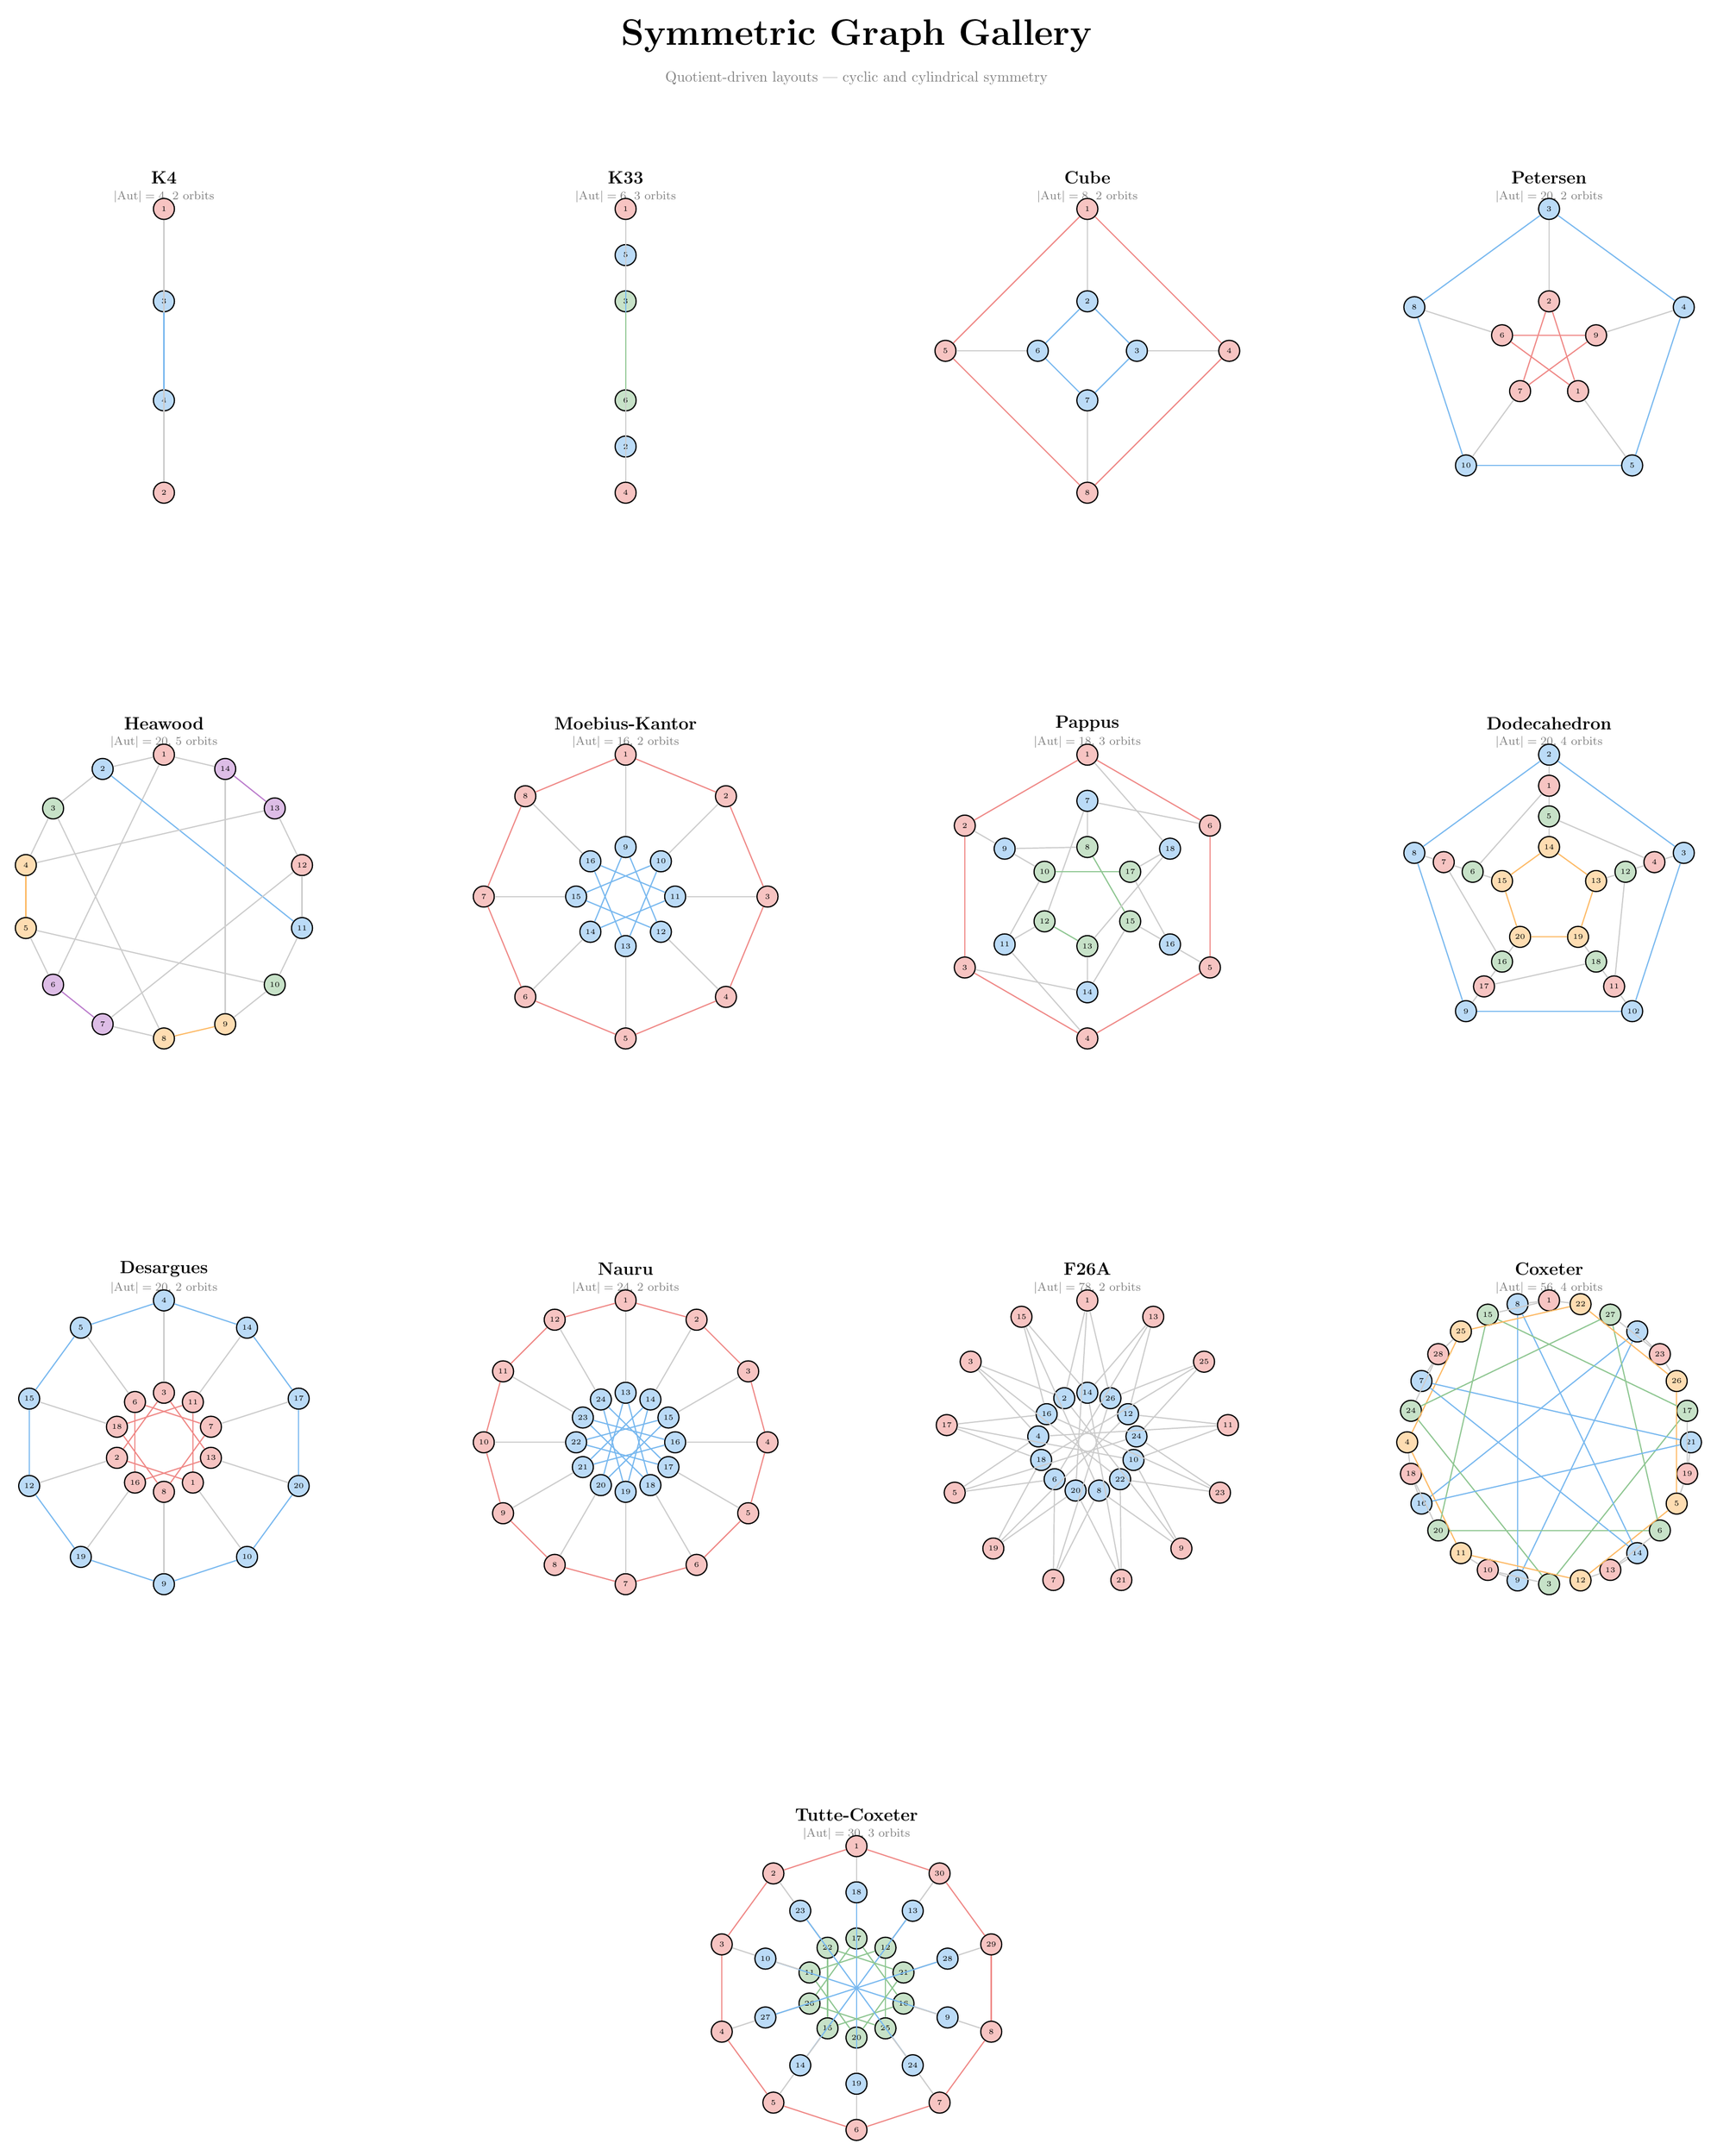
\begin{tikzpicture}[
  v/.style={circle, draw, thick, minimum size=5mm, inner sep=0pt},
  e/.style={thick, gray!40},
  graphtitle/.style={font=\large\bfseries},
  graphsub/.style={font=\footnotesize, text=gray},
]

\node[font=\Huge\bfseries] at (22.0, 7.5) {Symmetric Graph Gallery};
\node[font=\normalsize, text=gray] at (22.0, 6.5) {Quotient-driven layouts --- cyclic and cylindrical symmetry};

% === K4 ===
\node[graphtitle] at (5.5, 4.125) {K4};
\node[graphsub] at (5.5, 3.6750000000000003) {$|\mathrm{Aut}| = 4$, 2 orbits};
\node[v, fill=c0!30] (gK41) at (5.50, 3.38) {\tiny 1};
\node[v, fill=c0!30] (gK42) at (5.50, -3.38) {\tiny 2};
\node[v, fill=c1!30] (gK43) at (5.50, 1.18) {\tiny 3};
\node[v, fill=c1!30] (gK44) at (5.50, -1.18) {\tiny 4};
\draw[thick, c0!60] (gK41) -- (gK42);
\draw[e] (gK41) -- (gK43);
\draw[e] (gK41) -- (gK44);
\draw[e] (gK42) -- (gK43);
\draw[e] (gK42) -- (gK44);
\draw[thick, c1!60] (gK43) -- (gK44);

% === K33 ===
\node[graphtitle] at (16.5, 4.125) {K33};
\node[graphsub] at (16.5, 3.6750000000000003) {$|\mathrm{Aut}| = 6$, 3 orbits};
\node[v, fill=c0!30] (gK331) at (16.50, 3.38) {\tiny 1};
\node[v, fill=c1!30] (gK332) at (16.50, -2.28) {\tiny 2};
\node[v, fill=c2!30] (gK333) at (16.50, 1.18) {\tiny 3};
\node[v, fill=c0!30] (gK334) at (16.50, -3.38) {\tiny 4};
\node[v, fill=c1!30] (gK335) at (16.50, 2.28) {\tiny 5};
\node[v, fill=c2!30] (gK336) at (16.50, -1.18) {\tiny 6};
\draw[thick, c0!60] (gK331) -- (gK334);
\draw[e] (gK331) -- (gK335);
\draw[e] (gK331) -- (gK336);
\draw[e] (gK332) -- (gK334);
\draw[thick, c1!60] (gK332) -- (gK335);
\draw[e] (gK332) -- (gK336);
\draw[e] (gK333) -- (gK334);
\draw[e] (gK333) -- (gK335);
\draw[thick, c2!60] (gK333) -- (gK336);

% === Cube ===
\node[graphtitle] at (27.5, 4.125) {Cube};
\node[graphsub] at (27.5, 3.6750000000000003) {$|\mathrm{Aut}| = 8$, 2 orbits};
\node[v, fill=c0!30] (gCube1) at (27.50, 3.38) {\tiny 1};
\node[v, fill=c1!30] (gCube2) at (27.50, 1.18) {\tiny 2};
\node[v, fill=c1!30] (gCube3) at (28.68, -0.00) {\tiny 3};
\node[v, fill=c0!30] (gCube4) at (30.88, -0.00) {\tiny 4};
\node[v, fill=c0!30] (gCube5) at (24.12, 0.00) {\tiny 5};
\node[v, fill=c1!30] (gCube6) at (26.32, 0.00) {\tiny 6};
\node[v, fill=c1!30] (gCube7) at (27.50, -1.18) {\tiny 7};
\node[v, fill=c0!30] (gCube8) at (27.50, -3.38) {\tiny 8};
\draw[e] (gCube1) -- (gCube2);
\draw[thick, c0!60] (gCube1) -- (gCube4);
\draw[thick, c0!60] (gCube1) -- (gCube5);
\draw[thick, c1!60] (gCube2) -- (gCube3);
\draw[thick, c1!60] (gCube2) -- (gCube6);
\draw[e] (gCube3) -- (gCube4);
\draw[thick, c1!60] (gCube3) -- (gCube7);
\draw[thick, c0!60] (gCube4) -- (gCube8);
\draw[e] (gCube5) -- (gCube6);
\draw[thick, c0!60] (gCube5) -- (gCube8);
\draw[thick, c1!60] (gCube6) -- (gCube7);
\draw[e] (gCube7) -- (gCube8);

% === Petersen ===
\node[graphtitle] at (38.5, 4.125) {Petersen};
\node[graphsub] at (38.5, 3.6750000000000003) {$|\mathrm{Aut}| = 20$, 2 orbits};
\node[v, fill=c0!30] (gPetersen1) at (39.19, -0.96) {\tiny 1};
\node[v, fill=c0!30] (gPetersen2) at (38.50, 1.18) {\tiny 2};
\node[v, fill=c1!30] (gPetersen3) at (38.50, 3.38) {\tiny 3};
\node[v, fill=c1!30] (gPetersen4) at (41.71, 1.04) {\tiny 4};
\node[v, fill=c1!30] (gPetersen5) at (40.48, -2.73) {\tiny 5};
\node[v, fill=c0!30] (gPetersen6) at (37.38, 0.37) {\tiny 6};
\node[v, fill=c0!30] (gPetersen7) at (37.81, -0.96) {\tiny 7};
\node[v, fill=c1!30] (gPetersen8) at (35.29, 1.04) {\tiny 8};
\node[v, fill=c0!30] (gPetersen9) at (39.62, 0.37) {\tiny 9};
\node[v, fill=c1!30] (gPetersen10) at (36.52, -2.73) {\tiny 10};
\draw[thick, c0!60] (gPetersen1) -- (gPetersen2);
\draw[e] (gPetersen1) -- (gPetersen5);
\draw[thick, c0!60] (gPetersen1) -- (gPetersen6);
\draw[e] (gPetersen2) -- (gPetersen3);
\draw[thick, c0!60] (gPetersen2) -- (gPetersen7);
\draw[thick, c1!60] (gPetersen3) -- (gPetersen4);
\draw[thick, c1!60] (gPetersen3) -- (gPetersen8);
\draw[thick, c1!60] (gPetersen4) -- (gPetersen5);
\draw[e] (gPetersen4) -- (gPetersen9);
\draw[thick, c1!60] (gPetersen5) -- (gPetersen10);
\draw[e] (gPetersen6) -- (gPetersen8);
\draw[thick, c0!60] (gPetersen6) -- (gPetersen9);
\draw[thick, c0!60] (gPetersen7) -- (gPetersen9);
\draw[e] (gPetersen7) -- (gPetersen10);
\draw[thick, c1!60] (gPetersen8) -- (gPetersen10);

% === Heawood ===
\node[graphtitle] at (5.5, -8.875) {Heawood};
\node[graphsub] at (5.5, -9.325) {$|\mathrm{Aut}| = 20$, 5 orbits};
\node[v, fill=c0!30] (gHeawood1) at (5.50, -9.62) {\tiny 1};
\node[v, fill=c1!30] (gHeawood2) at (4.04, -9.96) {\tiny 2};
\node[v, fill=c2!30] (gHeawood3) at (2.86, -10.90) {\tiny 3};
\node[v, fill=c3!30] (gHeawood4) at (2.21, -12.25) {\tiny 4};
\node[v, fill=c3!30] (gHeawood5) at (2.21, -13.75) {\tiny 5};
\node[v, fill=c4!30] (gHeawood6) at (2.86, -15.10) {\tiny 6};
\node[v, fill=c4!30] (gHeawood7) at (4.04, -16.04) {\tiny 7};
\node[v, fill=c3!30] (gHeawood8) at (5.50, -16.38) {\tiny 8};
\node[v, fill=c3!30] (gHeawood9) at (6.96, -16.04) {\tiny 9};
\node[v, fill=c2!30] (gHeawood10) at (8.14, -15.10) {\tiny 10};
\node[v, fill=c1!30] (gHeawood11) at (8.79, -13.75) {\tiny 11};
\node[v, fill=c0!30] (gHeawood12) at (8.79, -12.25) {\tiny 12};
\node[v, fill=c4!30] (gHeawood13) at (8.14, -10.90) {\tiny 13};
\node[v, fill=c4!30] (gHeawood14) at (6.96, -9.96) {\tiny 14};
\draw[e] (gHeawood1) -- (gHeawood2);
\draw[e] (gHeawood1) -- (gHeawood6);
\draw[e] (gHeawood1) -- (gHeawood14);
\draw[e] (gHeawood2) -- (gHeawood3);
\draw[thick, c1!60] (gHeawood2) -- (gHeawood11);
\draw[e] (gHeawood3) -- (gHeawood4);
\draw[e] (gHeawood3) -- (gHeawood8);
\draw[thick, c3!60] (gHeawood4) -- (gHeawood5);
\draw[e] (gHeawood4) -- (gHeawood13);
\draw[e] (gHeawood5) -- (gHeawood6);
\draw[e] (gHeawood5) -- (gHeawood10);
\draw[thick, c4!60] (gHeawood6) -- (gHeawood7);
\draw[e] (gHeawood7) -- (gHeawood8);
\draw[e] (gHeawood7) -- (gHeawood12);
\draw[thick, c3!60] (gHeawood8) -- (gHeawood9);
\draw[e] (gHeawood9) -- (gHeawood10);
\draw[e] (gHeawood9) -- (gHeawood14);
\draw[e] (gHeawood10) -- (gHeawood11);
\draw[e] (gHeawood11) -- (gHeawood12);
\draw[e] (gHeawood12) -- (gHeawood13);
\draw[thick, c4!60] (gHeawood13) -- (gHeawood14);

% === Moebius-Kantor ===
\node[graphtitle] at (16.5, -8.875) {Moebius-Kantor};
\node[graphsub] at (16.5, -9.325) {$|\mathrm{Aut}| = 16$, 2 orbits};
\node[v, fill=c0!30] (gMoebius-Kantor1) at (16.50, -9.62) {\tiny 1};
\node[v, fill=c0!30] (gMoebius-Kantor2) at (18.89, -10.61) {\tiny 2};
\node[v, fill=c0!30] (gMoebius-Kantor3) at (19.88, -13.00) {\tiny 3};
\node[v, fill=c0!30] (gMoebius-Kantor4) at (18.89, -15.39) {\tiny 4};
\node[v, fill=c0!30] (gMoebius-Kantor5) at (16.50, -16.38) {\tiny 5};
\node[v, fill=c0!30] (gMoebius-Kantor6) at (14.11, -15.39) {\tiny 6};
\node[v, fill=c0!30] (gMoebius-Kantor7) at (13.12, -13.00) {\tiny 7};
\node[v, fill=c0!30] (gMoebius-Kantor8) at (14.11, -10.61) {\tiny 8};
\node[v, fill=c1!30] (gMoebius-Kantor9) at (16.50, -11.82) {\tiny 9};
\node[v, fill=c1!30] (gMoebius-Kantor10) at (17.34, -12.16) {\tiny 10};
\node[v, fill=c1!30] (gMoebius-Kantor11) at (17.68, -13.00) {\tiny 11};
\node[v, fill=c1!30] (gMoebius-Kantor12) at (17.34, -13.84) {\tiny 12};
\node[v, fill=c1!30] (gMoebius-Kantor13) at (16.50, -14.18) {\tiny 13};
\node[v, fill=c1!30] (gMoebius-Kantor14) at (15.66, -13.84) {\tiny 14};
\node[v, fill=c1!30] (gMoebius-Kantor15) at (15.32, -13.00) {\tiny 15};
\node[v, fill=c1!30] (gMoebius-Kantor16) at (15.66, -12.16) {\tiny 16};
\draw[thick, c0!60] (gMoebius-Kantor1) -- (gMoebius-Kantor2);
\draw[thick, c0!60] (gMoebius-Kantor1) -- (gMoebius-Kantor8);
\draw[e] (gMoebius-Kantor1) -- (gMoebius-Kantor9);
\draw[thick, c0!60] (gMoebius-Kantor2) -- (gMoebius-Kantor3);
\draw[e] (gMoebius-Kantor2) -- (gMoebius-Kantor10);
\draw[thick, c0!60] (gMoebius-Kantor3) -- (gMoebius-Kantor4);
\draw[e] (gMoebius-Kantor3) -- (gMoebius-Kantor11);
\draw[thick, c0!60] (gMoebius-Kantor4) -- (gMoebius-Kantor5);
\draw[e] (gMoebius-Kantor4) -- (gMoebius-Kantor12);
\draw[thick, c0!60] (gMoebius-Kantor5) -- (gMoebius-Kantor6);
\draw[e] (gMoebius-Kantor5) -- (gMoebius-Kantor13);
\draw[thick, c0!60] (gMoebius-Kantor6) -- (gMoebius-Kantor7);
\draw[e] (gMoebius-Kantor6) -- (gMoebius-Kantor14);
\draw[thick, c0!60] (gMoebius-Kantor7) -- (gMoebius-Kantor8);
\draw[e] (gMoebius-Kantor7) -- (gMoebius-Kantor15);
\draw[e] (gMoebius-Kantor8) -- (gMoebius-Kantor16);
\draw[thick, c1!60] (gMoebius-Kantor9) -- (gMoebius-Kantor12);
\draw[thick, c1!60] (gMoebius-Kantor9) -- (gMoebius-Kantor14);
\draw[thick, c1!60] (gMoebius-Kantor10) -- (gMoebius-Kantor13);
\draw[thick, c1!60] (gMoebius-Kantor10) -- (gMoebius-Kantor15);
\draw[thick, c1!60] (gMoebius-Kantor11) -- (gMoebius-Kantor14);
\draw[thick, c1!60] (gMoebius-Kantor11) -- (gMoebius-Kantor16);
\draw[thick, c1!60] (gMoebius-Kantor12) -- (gMoebius-Kantor15);
\draw[thick, c1!60] (gMoebius-Kantor13) -- (gMoebius-Kantor16);

% === Pappus ===
\node[graphtitle] at (27.5, -8.875) {Pappus};
\node[graphsub] at (27.5, -9.325) {$|\mathrm{Aut}| = 18$, 3 orbits};
\node[v, fill=c0!30] (gPappus1) at (27.50, -9.62) {\tiny 1};
\node[v, fill=c0!30] (gPappus2) at (24.58, -11.31) {\tiny 2};
\node[v, fill=c0!30] (gPappus3) at (24.58, -14.69) {\tiny 3};
\node[v, fill=c0!30] (gPappus4) at (27.50, -16.38) {\tiny 4};
\node[v, fill=c0!30] (gPappus5) at (30.42, -14.69) {\tiny 5};
\node[v, fill=c0!30] (gPappus6) at (30.42, -11.31) {\tiny 6};
\node[v, fill=c1!30] (gPappus7) at (27.50, -10.72) {\tiny 7};
\node[v, fill=c2!30] (gPappus8) at (27.50, -11.82) {\tiny 8};
\node[v, fill=c1!30] (gPappus9) at (25.53, -11.86) {\tiny 9};
\node[v, fill=c2!30] (gPappus10) at (26.48, -12.41) {\tiny 10};
\node[v, fill=c1!30] (gPappus11) at (25.53, -14.14) {\tiny 11};
\node[v, fill=c2!30] (gPappus12) at (26.48, -13.59) {\tiny 12};
\node[v, fill=c2!30] (gPappus13) at (27.50, -14.18) {\tiny 13};
\node[v, fill=c1!30] (gPappus14) at (27.50, -15.28) {\tiny 14};
\node[v, fill=c2!30] (gPappus15) at (28.52, -13.59) {\tiny 15};
\node[v, fill=c1!30] (gPappus16) at (29.47, -14.14) {\tiny 16};
\node[v, fill=c2!30] (gPappus17) at (28.52, -12.41) {\tiny 17};
\node[v, fill=c1!30] (gPappus18) at (29.47, -11.86) {\tiny 18};
\draw[thick, c0!60] (gPappus1) -- (gPappus2);
\draw[thick, c0!60] (gPappus1) -- (gPappus6);
\draw[e] (gPappus1) -- (gPappus18);
\draw[thick, c0!60] (gPappus2) -- (gPappus3);
\draw[e] (gPappus2) -- (gPappus9);
\draw[thick, c0!60] (gPappus3) -- (gPappus4);
\draw[e] (gPappus3) -- (gPappus14);
\draw[thick, c0!60] (gPappus4) -- (gPappus5);
\draw[e] (gPappus4) -- (gPappus11);
\draw[thick, c0!60] (gPappus5) -- (gPappus6);
\draw[e] (gPappus5) -- (gPappus16);
\draw[e] (gPappus6) -- (gPappus7);
\draw[e] (gPappus7) -- (gPappus8);
\draw[e] (gPappus7) -- (gPappus12);
\draw[e] (gPappus8) -- (gPappus9);
\draw[thick, c2!60] (gPappus8) -- (gPappus15);
\draw[e] (gPappus9) -- (gPappus10);
\draw[e] (gPappus10) -- (gPappus11);
\draw[thick, c2!60] (gPappus10) -- (gPappus17);
\draw[e] (gPappus11) -- (gPappus12);
\draw[thick, c2!60] (gPappus12) -- (gPappus13);
\draw[e] (gPappus13) -- (gPappus14);
\draw[e] (gPappus13) -- (gPappus18);
\draw[e] (gPappus14) -- (gPappus15);
\draw[e] (gPappus15) -- (gPappus16);
\draw[e] (gPappus16) -- (gPappus17);
\draw[e] (gPappus17) -- (gPappus18);

% === Dodecahedron ===
\node[graphtitle] at (38.5, -8.875) {Dodecahedron};
\node[graphsub] at (38.5, -9.325) {$|\mathrm{Aut}| = 20$, 4 orbits};
\node[v, fill=c0!30] (gDodecahedron1) at (38.50, -10.36) {\tiny 1};
\node[v, fill=c1!30] (gDodecahedron2) at (38.50, -9.62) {\tiny 2};
\node[v, fill=c1!30] (gDodecahedron3) at (41.71, -11.96) {\tiny 3};
\node[v, fill=c0!30] (gDodecahedron4) at (41.01, -12.18) {\tiny 4};
\node[v, fill=c2!30] (gDodecahedron5) at (38.50, -11.09) {\tiny 5};
\node[v, fill=c2!30] (gDodecahedron6) at (36.68, -12.41) {\tiny 6};
\node[v, fill=c0!30] (gDodecahedron7) at (35.99, -12.18) {\tiny 7};
\node[v, fill=c1!30] (gDodecahedron8) at (35.29, -11.96) {\tiny 8};
\node[v, fill=c1!30] (gDodecahedron9) at (36.52, -15.73) {\tiny 9};
\node[v, fill=c1!30] (gDodecahedron10) at (40.48, -15.73) {\tiny 10};
\node[v, fill=c0!30] (gDodecahedron11) at (40.05, -15.14) {\tiny 11};
\node[v, fill=c2!30] (gDodecahedron12) at (40.32, -12.41) {\tiny 12};
\node[v, fill=c3!30] (gDodecahedron13) at (39.62, -12.63) {\tiny 13};
\node[v, fill=c3!30] (gDodecahedron14) at (38.50, -11.82) {\tiny 14};
\node[v, fill=c3!30] (gDodecahedron15) at (37.38, -12.63) {\tiny 15};
\node[v, fill=c2!30] (gDodecahedron16) at (37.38, -14.55) {\tiny 16};
\node[v, fill=c0!30] (gDodecahedron17) at (36.95, -15.14) {\tiny 17};
\node[v, fill=c2!30] (gDodecahedron18) at (39.62, -14.55) {\tiny 18};
\node[v, fill=c3!30] (gDodecahedron19) at (39.19, -13.96) {\tiny 19};
\node[v, fill=c3!30] (gDodecahedron20) at (37.81, -13.96) {\tiny 20};
\draw[e] (gDodecahedron1) -- (gDodecahedron2);
\draw[e] (gDodecahedron1) -- (gDodecahedron5);
\draw[e] (gDodecahedron1) -- (gDodecahedron6);
\draw[thick, c1!60] (gDodecahedron2) -- (gDodecahedron3);
\draw[thick, c1!60] (gDodecahedron2) -- (gDodecahedron8);
\draw[e] (gDodecahedron3) -- (gDodecahedron4);
\draw[thick, c1!60] (gDodecahedron3) -- (gDodecahedron10);
\draw[e] (gDodecahedron4) -- (gDodecahedron5);
\draw[e] (gDodecahedron4) -- (gDodecahedron12);
\draw[e] (gDodecahedron5) -- (gDodecahedron14);
\draw[e] (gDodecahedron6) -- (gDodecahedron7);
\draw[e] (gDodecahedron6) -- (gDodecahedron15);
\draw[e] (gDodecahedron7) -- (gDodecahedron8);
\draw[e] (gDodecahedron7) -- (gDodecahedron16);
\draw[thick, c1!60] (gDodecahedron8) -- (gDodecahedron9);
\draw[thick, c1!60] (gDodecahedron9) -- (gDodecahedron10);
\draw[e] (gDodecahedron9) -- (gDodecahedron17);
\draw[e] (gDodecahedron10) -- (gDodecahedron11);
\draw[e] (gDodecahedron11) -- (gDodecahedron12);
\draw[e] (gDodecahedron11) -- (gDodecahedron18);
\draw[e] (gDodecahedron12) -- (gDodecahedron13);
\draw[thick, c3!60] (gDodecahedron13) -- (gDodecahedron14);
\draw[thick, c3!60] (gDodecahedron13) -- (gDodecahedron19);
\draw[thick, c3!60] (gDodecahedron14) -- (gDodecahedron15);
\draw[thick, c3!60] (gDodecahedron15) -- (gDodecahedron20);
\draw[e] (gDodecahedron16) -- (gDodecahedron17);
\draw[e] (gDodecahedron16) -- (gDodecahedron20);
\draw[e] (gDodecahedron17) -- (gDodecahedron18);
\draw[e] (gDodecahedron18) -- (gDodecahedron19);
\draw[thick, c3!60] (gDodecahedron19) -- (gDodecahedron20);

% === Desargues ===
\node[graphtitle] at (5.5, -21.875) {Desargues};
\node[graphsub] at (5.5, -22.325) {$|\mathrm{Aut}| = 20$, 2 orbits};
\node[v, fill=c0!30] (gDesargues1) at (6.19, -26.96) {\tiny 1};
\node[v, fill=c0!30] (gDesargues2) at (4.38, -26.37) {\tiny 2};
\node[v, fill=c0!30] (gDesargues3) at (5.50, -24.82) {\tiny 3};
\node[v, fill=c1!30] (gDesargues4) at (5.50, -22.62) {\tiny 4};
\node[v, fill=c1!30] (gDesargues5) at (3.52, -23.27) {\tiny 5};
\node[v, fill=c0!30] (gDesargues6) at (4.81, -25.04) {\tiny 6};
\node[v, fill=c0!30] (gDesargues7) at (6.62, -25.63) {\tiny 7};
\node[v, fill=c0!30] (gDesargues8) at (5.50, -27.18) {\tiny 8};
\node[v, fill=c1!30] (gDesargues9) at (5.50, -29.38) {\tiny 9};
\node[v, fill=c1!30] (gDesargues10) at (7.48, -28.73) {\tiny 10};
\node[v, fill=c0!30] (gDesargues11) at (6.19, -25.04) {\tiny 11};
\node[v, fill=c1!30] (gDesargues12) at (2.29, -27.04) {\tiny 12};
\node[v, fill=c0!30] (gDesargues13) at (6.62, -26.37) {\tiny 13};
\node[v, fill=c1!30] (gDesargues14) at (7.48, -23.27) {\tiny 14};
\node[v, fill=c1!30] (gDesargues15) at (2.29, -24.96) {\tiny 15};
\node[v, fill=c0!30] (gDesargues16) at (4.81, -26.96) {\tiny 16};
\node[v, fill=c1!30] (gDesargues17) at (8.71, -24.96) {\tiny 17};
\node[v, fill=c0!30] (gDesargues18) at (4.38, -25.63) {\tiny 18};
\node[v, fill=c1!30] (gDesargues19) at (3.52, -28.73) {\tiny 19};
\node[v, fill=c1!30] (gDesargues20) at (8.71, -27.04) {\tiny 20};
\draw[thick, c0!60] (gDesargues1) -- (gDesargues2);
\draw[e] (gDesargues1) -- (gDesargues10);
\draw[thick, c0!60] (gDesargues1) -- (gDesargues11);
\draw[thick, c0!60] (gDesargues2) -- (gDesargues3);
\draw[e] (gDesargues2) -- (gDesargues12);
\draw[e] (gDesargues3) -- (gDesargues4);
\draw[thick, c0!60] (gDesargues3) -- (gDesargues13);
\draw[thick, c1!60] (gDesargues4) -- (gDesargues5);
\draw[thick, c1!60] (gDesargues4) -- (gDesargues14);
\draw[e] (gDesargues5) -- (gDesargues6);
\draw[thick, c1!60] (gDesargues5) -- (gDesargues15);
\draw[thick, c0!60] (gDesargues6) -- (gDesargues7);
\draw[thick, c0!60] (gDesargues6) -- (gDesargues16);
\draw[thick, c0!60] (gDesargues7) -- (gDesargues8);
\draw[e] (gDesargues7) -- (gDesargues17);
\draw[e] (gDesargues8) -- (gDesargues9);
\draw[thick, c0!60] (gDesargues8) -- (gDesargues18);
\draw[thick, c1!60] (gDesargues9) -- (gDesargues10);
\draw[thick, c1!60] (gDesargues9) -- (gDesargues19);
\draw[thick, c1!60] (gDesargues10) -- (gDesargues20);
\draw[e] (gDesargues11) -- (gDesargues14);
\draw[thick, c0!60] (gDesargues11) -- (gDesargues18);
\draw[thick, c1!60] (gDesargues12) -- (gDesargues15);
\draw[thick, c1!60] (gDesargues12) -- (gDesargues19);
\draw[thick, c0!60] (gDesargues13) -- (gDesargues16);
\draw[e] (gDesargues13) -- (gDesargues20);
\draw[thick, c1!60] (gDesargues14) -- (gDesargues17);
\draw[e] (gDesargues15) -- (gDesargues18);
\draw[e] (gDesargues16) -- (gDesargues19);
\draw[thick, c1!60] (gDesargues17) -- (gDesargues20);

% === Nauru ===
\node[graphtitle] at (16.5, -21.875) {Nauru};
\node[graphsub] at (16.5, -22.325) {$|\mathrm{Aut}| = 24$, 2 orbits};
\node[v, fill=c0!30] (gNauru1) at (16.50, -22.62) {\tiny 1};
\node[v, fill=c0!30] (gNauru2) at (18.19, -23.08) {\tiny 2};
\node[v, fill=c0!30] (gNauru3) at (19.42, -24.31) {\tiny 3};
\node[v, fill=c0!30] (gNauru4) at (19.88, -26.00) {\tiny 4};
\node[v, fill=c0!30] (gNauru5) at (19.42, -27.69) {\tiny 5};
\node[v, fill=c0!30] (gNauru6) at (18.19, -28.92) {\tiny 6};
\node[v, fill=c0!30] (gNauru7) at (16.50, -29.38) {\tiny 7};
\node[v, fill=c0!30] (gNauru8) at (14.81, -28.92) {\tiny 8};
\node[v, fill=c0!30] (gNauru9) at (13.58, -27.69) {\tiny 9};
\node[v, fill=c0!30] (gNauru10) at (13.12, -26.00) {\tiny 10};
\node[v, fill=c0!30] (gNauru11) at (13.58, -24.31) {\tiny 11};
\node[v, fill=c0!30] (gNauru12) at (14.81, -23.08) {\tiny 12};
\node[v, fill=c1!30] (gNauru13) at (16.50, -24.82) {\tiny 13};
\node[v, fill=c1!30] (gNauru14) at (17.09, -24.98) {\tiny 14};
\node[v, fill=c1!30] (gNauru15) at (17.52, -25.41) {\tiny 15};
\node[v, fill=c1!30] (gNauru16) at (17.68, -26.00) {\tiny 16};
\node[v, fill=c1!30] (gNauru17) at (17.52, -26.59) {\tiny 17};
\node[v, fill=c1!30] (gNauru18) at (17.09, -27.02) {\tiny 18};
\node[v, fill=c1!30] (gNauru19) at (16.50, -27.18) {\tiny 19};
\node[v, fill=c1!30] (gNauru20) at (15.91, -27.02) {\tiny 20};
\node[v, fill=c1!30] (gNauru21) at (15.48, -26.59) {\tiny 21};
\node[v, fill=c1!30] (gNauru22) at (15.32, -26.00) {\tiny 22};
\node[v, fill=c1!30] (gNauru23) at (15.48, -25.41) {\tiny 23};
\node[v, fill=c1!30] (gNauru24) at (15.91, -24.98) {\tiny 24};
\draw[thick, c0!60] (gNauru1) -- (gNauru2);
\draw[thick, c0!60] (gNauru1) -- (gNauru12);
\draw[e] (gNauru1) -- (gNauru13);
\draw[thick, c0!60] (gNauru2) -- (gNauru3);
\draw[e] (gNauru2) -- (gNauru14);
\draw[thick, c0!60] (gNauru3) -- (gNauru4);
\draw[e] (gNauru3) -- (gNauru15);
\draw[thick, c0!60] (gNauru4) -- (gNauru5);
\draw[e] (gNauru4) -- (gNauru16);
\draw[thick, c0!60] (gNauru5) -- (gNauru6);
\draw[e] (gNauru5) -- (gNauru17);
\draw[thick, c0!60] (gNauru6) -- (gNauru7);
\draw[e] (gNauru6) -- (gNauru18);
\draw[thick, c0!60] (gNauru7) -- (gNauru8);
\draw[e] (gNauru7) -- (gNauru19);
\draw[thick, c0!60] (gNauru8) -- (gNauru9);
\draw[e] (gNauru8) -- (gNauru20);
\draw[thick, c0!60] (gNauru9) -- (gNauru10);
\draw[e] (gNauru9) -- (gNauru21);
\draw[thick, c0!60] (gNauru10) -- (gNauru11);
\draw[e] (gNauru10) -- (gNauru22);
\draw[thick, c0!60] (gNauru11) -- (gNauru12);
\draw[e] (gNauru11) -- (gNauru23);
\draw[e] (gNauru12) -- (gNauru24);
\draw[thick, c1!60] (gNauru13) -- (gNauru18);
\draw[thick, c1!60] (gNauru13) -- (gNauru20);
\draw[thick, c1!60] (gNauru14) -- (gNauru19);
\draw[thick, c1!60] (gNauru14) -- (gNauru21);
\draw[thick, c1!60] (gNauru15) -- (gNauru20);
\draw[thick, c1!60] (gNauru15) -- (gNauru22);
\draw[thick, c1!60] (gNauru16) -- (gNauru21);
\draw[thick, c1!60] (gNauru16) -- (gNauru23);
\draw[thick, c1!60] (gNauru17) -- (gNauru22);
\draw[thick, c1!60] (gNauru17) -- (gNauru24);
\draw[thick, c1!60] (gNauru18) -- (gNauru23);
\draw[thick, c1!60] (gNauru19) -- (gNauru24);

% === F26A ===
\node[graphtitle] at (27.5, -21.875) {F26A};
\node[graphsub] at (27.5, -22.325) {$|\mathrm{Aut}| = 78$, 2 orbits};
\node[v, fill=c0!30] (gF26A1) at (27.50, -22.62) {\tiny 1};
\node[v, fill=c1!30] (gF26A2) at (26.95, -24.95) {\tiny 2};
\node[v, fill=c0!30] (gF26A3) at (24.72, -24.08) {\tiny 3};
\node[v, fill=c1!30] (gF26A4) at (26.33, -25.86) {\tiny 4};
\node[v, fill=c0!30] (gF26A5) at (24.34, -27.20) {\tiny 5};
\node[v, fill=c1!30] (gF26A6) at (26.72, -26.88) {\tiny 6};
\node[v, fill=c0!30] (gF26A7) at (26.69, -29.28) {\tiny 7};
\node[v, fill=c1!30] (gF26A8) at (27.78, -27.15) {\tiny 8};
\node[v, fill=c0!30] (gF26A9) at (29.74, -28.53) {\tiny 9};
\node[v, fill=c1!30] (gF26A10) at (28.60, -26.42) {\tiny 10};
\node[v, fill=c0!30] (gF26A11) at (30.85, -25.59) {\tiny 11};
\node[v, fill=c1!30] (gF26A12) at (28.47, -25.33) {\tiny 12};
\node[v, fill=c0!30] (gF26A13) at (29.07, -23.01) {\tiny 13};
\node[v, fill=c1!30] (gF26A14) at (27.50, -24.82) {\tiny 14};
\node[v, fill=c0!30] (gF26A15) at (25.93, -23.01) {\tiny 15};
\node[v, fill=c1!30] (gF26A16) at (26.53, -25.33) {\tiny 16};
\node[v, fill=c0!30] (gF26A17) at (24.15, -25.59) {\tiny 17};
\node[v, fill=c1!30] (gF26A18) at (26.40, -26.42) {\tiny 18};
\node[v, fill=c0!30] (gF26A19) at (25.26, -28.53) {\tiny 19};
\node[v, fill=c1!30] (gF26A20) at (27.22, -27.15) {\tiny 20};
\node[v, fill=c0!30] (gF26A21) at (28.31, -29.28) {\tiny 21};
\node[v, fill=c1!30] (gF26A22) at (28.28, -26.88) {\tiny 22};
\node[v, fill=c0!30] (gF26A23) at (30.66, -27.20) {\tiny 23};
\node[v, fill=c1!30] (gF26A24) at (28.67, -25.86) {\tiny 24};
\node[v, fill=c0!30] (gF26A25) at (30.28, -24.08) {\tiny 25};
\node[v, fill=c1!30] (gF26A26) at (28.05, -24.95) {\tiny 26};
\draw[e] (gF26A1) -- (gF26A2);
\draw[e] (gF26A1) -- (gF26A26);
\draw[e] (gF26A1) -- (gF26A20);
\draw[e] (gF26A2) -- (gF26A3);
\draw[e] (gF26A2) -- (gF26A9);
\draw[e] (gF26A3) -- (gF26A4);
\draw[e] (gF26A3) -- (gF26A22);
\draw[e] (gF26A4) -- (gF26A5);
\draw[e] (gF26A4) -- (gF26A11);
\draw[e] (gF26A5) -- (gF26A6);
\draw[e] (gF26A5) -- (gF26A24);
\draw[e] (gF26A6) -- (gF26A7);
\draw[e] (gF26A6) -- (gF26A13);
\draw[e] (gF26A7) -- (gF26A8);
\draw[e] (gF26A7) -- (gF26A26);
\draw[e] (gF26A8) -- (gF26A9);
\draw[e] (gF26A8) -- (gF26A15);
\draw[e] (gF26A9) -- (gF26A10);
\draw[e] (gF26A10) -- (gF26A11);
\draw[e] (gF26A10) -- (gF26A17);
\draw[e] (gF26A11) -- (gF26A12);
\draw[e] (gF26A12) -- (gF26A13);
\draw[e] (gF26A12) -- (gF26A19);
\draw[e] (gF26A13) -- (gF26A14);
\draw[e] (gF26A14) -- (gF26A15);
\draw[e] (gF26A14) -- (gF26A21);
\draw[e] (gF26A15) -- (gF26A16);
\draw[e] (gF26A16) -- (gF26A17);
\draw[e] (gF26A16) -- (gF26A23);
\draw[e] (gF26A17) -- (gF26A18);
\draw[e] (gF26A18) -- (gF26A19);
\draw[e] (gF26A18) -- (gF26A25);
\draw[e] (gF26A19) -- (gF26A20);
\draw[e] (gF26A20) -- (gF26A21);
\draw[e] (gF26A21) -- (gF26A22);
\draw[e] (gF26A22) -- (gF26A23);
\draw[e] (gF26A23) -- (gF26A24);
\draw[e] (gF26A24) -- (gF26A25);
\draw[e] (gF26A25) -- (gF26A26);

% === Coxeter ===
\node[graphtitle] at (38.5, -21.875) {Coxeter};
\node[graphsub] at (38.5, -22.325) {$|\mathrm{Aut}| = 56$, 4 orbits};
\node[v, fill=c0!30] (gCoxeter1) at (38.50, -22.62) {\tiny 1};
\node[v, fill=c1!30] (gCoxeter2) at (40.60, -23.36) {\tiny 2};
\node[v, fill=c2!30] (gCoxeter3) at (38.50, -29.38) {\tiny 3};
\node[v, fill=c3!30] (gCoxeter4) at (35.12, -26.00) {\tiny 4};
\node[v, fill=c3!30] (gCoxeter5) at (41.54, -27.46) {\tiny 5};
\node[v, fill=c2!30] (gCoxeter6) at (41.14, -28.10) {\tiny 6};
\node[v, fill=c1!30] (gCoxeter7) at (35.46, -24.54) {\tiny 7};
\node[v, fill=c1!30] (gCoxeter8) at (37.75, -22.71) {\tiny 8};
\node[v, fill=c1!30] (gCoxeter9) at (37.75, -29.29) {\tiny 9};
\node[v, fill=c0!30] (gCoxeter10) at (37.04, -29.04) {\tiny 10};
\node[v, fill=c3!30] (gCoxeter11) at (36.40, -28.64) {\tiny 11};
\node[v, fill=c3!30] (gCoxeter12) at (39.25, -29.29) {\tiny 12};
\node[v, fill=c0!30] (gCoxeter13) at (39.96, -29.04) {\tiny 13};
\node[v, fill=c1!30] (gCoxeter14) at (40.60, -28.64) {\tiny 14};
\node[v, fill=c2!30] (gCoxeter15) at (37.04, -22.96) {\tiny 15};
\node[v, fill=c1!30] (gCoxeter16) at (35.46, -27.46) {\tiny 16};
\node[v, fill=c2!30] (gCoxeter17) at (41.79, -25.25) {\tiny 17};
\node[v, fill=c0!30] (gCoxeter18) at (35.21, -26.75) {\tiny 18};
\node[v, fill=c0!30] (gCoxeter19) at (41.79, -26.75) {\tiny 19};
\node[v, fill=c2!30] (gCoxeter20) at (35.86, -28.10) {\tiny 20};
\node[v, fill=c1!30] (gCoxeter21) at (41.88, -26.00) {\tiny 21};
\node[v, fill=c3!30] (gCoxeter22) at (39.25, -22.71) {\tiny 22};
\node[v, fill=c0!30] (gCoxeter23) at (41.14, -23.90) {\tiny 23};
\node[v, fill=c2!30] (gCoxeter24) at (35.21, -25.25) {\tiny 24};
\node[v, fill=c3!30] (gCoxeter25) at (36.40, -23.36) {\tiny 25};
\node[v, fill=c3!30] (gCoxeter26) at (41.54, -24.54) {\tiny 26};
\node[v, fill=c2!30] (gCoxeter27) at (39.96, -22.96) {\tiny 27};
\node[v, fill=c0!30] (gCoxeter28) at (35.86, -23.90) {\tiny 28};
\draw[e] (gCoxeter1) -- (gCoxeter8);
\draw[e] (gCoxeter1) -- (gCoxeter15);
\draw[e] (gCoxeter1) -- (gCoxeter22);
\draw[thick, c1!60] (gCoxeter2) -- (gCoxeter9);
\draw[thick, c1!60] (gCoxeter2) -- (gCoxeter16);
\draw[e] (gCoxeter2) -- (gCoxeter23);
\draw[e] (gCoxeter3) -- (gCoxeter10);
\draw[thick, c2!60] (gCoxeter3) -- (gCoxeter17);
\draw[thick, c2!60] (gCoxeter3) -- (gCoxeter24);
\draw[thick, c3!60] (gCoxeter4) -- (gCoxeter11);
\draw[e] (gCoxeter4) -- (gCoxeter18);
\draw[thick, c3!60] (gCoxeter4) -- (gCoxeter25);
\draw[thick, c3!60] (gCoxeter5) -- (gCoxeter12);
\draw[e] (gCoxeter5) -- (gCoxeter19);
\draw[thick, c3!60] (gCoxeter5) -- (gCoxeter26);
\draw[e] (gCoxeter6) -- (gCoxeter13);
\draw[thick, c2!60] (gCoxeter6) -- (gCoxeter20);
\draw[thick, c2!60] (gCoxeter6) -- (gCoxeter27);
\draw[thick, c1!60] (gCoxeter7) -- (gCoxeter14);
\draw[thick, c1!60] (gCoxeter7) -- (gCoxeter21);
\draw[e] (gCoxeter7) -- (gCoxeter28);
\draw[thick, c1!60] (gCoxeter8) -- (gCoxeter9);
\draw[thick, c1!60] (gCoxeter8) -- (gCoxeter14);
\draw[e] (gCoxeter9) -- (gCoxeter10);
\draw[e] (gCoxeter10) -- (gCoxeter11);
\draw[thick, c3!60] (gCoxeter11) -- (gCoxeter12);
\draw[e] (gCoxeter12) -- (gCoxeter13);
\draw[e] (gCoxeter13) -- (gCoxeter14);
\draw[thick, c2!60] (gCoxeter15) -- (gCoxeter17);
\draw[thick, c2!60] (gCoxeter15) -- (gCoxeter20);
\draw[e] (gCoxeter16) -- (gCoxeter18);
\draw[thick, c1!60] (gCoxeter16) -- (gCoxeter21);
\draw[e] (gCoxeter17) -- (gCoxeter19);
\draw[e] (gCoxeter18) -- (gCoxeter20);
\draw[e] (gCoxeter19) -- (gCoxeter21);
\draw[thick, c3!60] (gCoxeter22) -- (gCoxeter25);
\draw[thick, c3!60] (gCoxeter22) -- (gCoxeter26);
\draw[e] (gCoxeter23) -- (gCoxeter26);
\draw[e] (gCoxeter23) -- (gCoxeter27);
\draw[thick, c2!60] (gCoxeter24) -- (gCoxeter27);
\draw[e] (gCoxeter24) -- (gCoxeter28);
\draw[e] (gCoxeter25) -- (gCoxeter28);

% === Tutte-Coxeter ===
\node[graphtitle] at (22.0, -34.875) {Tutte-Coxeter};
\node[graphsub] at (22.0, -35.325) {$|\mathrm{Aut}| = 30$, 3 orbits};
\node[v, fill=c0!30] (gTutte-Coxeter1) at (22.00, -35.62) {\tiny 1};
\node[v, fill=c0!30] (gTutte-Coxeter2) at (20.02, -36.27) {\tiny 2};
\node[v, fill=c0!30] (gTutte-Coxeter3) at (18.79, -37.96) {\tiny 3};
\node[v, fill=c0!30] (gTutte-Coxeter4) at (18.79, -40.04) {\tiny 4};
\node[v, fill=c0!30] (gTutte-Coxeter5) at (20.02, -41.73) {\tiny 5};
\node[v, fill=c0!30] (gTutte-Coxeter6) at (22.00, -42.38) {\tiny 6};
\node[v, fill=c0!30] (gTutte-Coxeter7) at (23.98, -41.73) {\tiny 7};
\node[v, fill=c0!30] (gTutte-Coxeter8) at (25.21, -40.04) {\tiny 8};
\node[v, fill=c1!30] (gTutte-Coxeter9) at (24.17, -39.70) {\tiny 9};
\node[v, fill=c1!30] (gTutte-Coxeter10) at (19.83, -38.30) {\tiny 10};
\node[v, fill=c2!30] (gTutte-Coxeter11) at (20.88, -38.63) {\tiny 11};
\node[v, fill=c2!30] (gTutte-Coxeter12) at (22.69, -38.04) {\tiny 12};
\node[v, fill=c1!30] (gTutte-Coxeter13) at (23.34, -37.16) {\tiny 13};
\node[v, fill=c1!30] (gTutte-Coxeter14) at (20.66, -40.84) {\tiny 14};
\node[v, fill=c2!30] (gTutte-Coxeter15) at (21.31, -39.96) {\tiny 15};
\node[v, fill=c2!30] (gTutte-Coxeter16) at (23.12, -39.37) {\tiny 16};
\node[v, fill=c2!30] (gTutte-Coxeter17) at (22.00, -37.82) {\tiny 17};
\node[v, fill=c1!30] (gTutte-Coxeter18) at (22.00, -36.72) {\tiny 18};
\node[v, fill=c1!30] (gTutte-Coxeter19) at (22.00, -41.28) {\tiny 19};
\node[v, fill=c2!30] (gTutte-Coxeter20) at (22.00, -40.18) {\tiny 20};
\node[v, fill=c2!30] (gTutte-Coxeter21) at (23.12, -38.63) {\tiny 21};
\node[v, fill=c2!30] (gTutte-Coxeter22) at (21.31, -38.04) {\tiny 22};
\node[v, fill=c1!30] (gTutte-Coxeter23) at (20.66, -37.16) {\tiny 23};
\node[v, fill=c1!30] (gTutte-Coxeter24) at (23.34, -40.84) {\tiny 24};
\node[v, fill=c2!30] (gTutte-Coxeter25) at (22.69, -39.96) {\tiny 25};
\node[v, fill=c2!30] (gTutte-Coxeter26) at (20.88, -39.37) {\tiny 26};
\node[v, fill=c1!30] (gTutte-Coxeter27) at (19.83, -39.70) {\tiny 27};
\node[v, fill=c1!30] (gTutte-Coxeter28) at (24.17, -38.30) {\tiny 28};
\node[v, fill=c0!30] (gTutte-Coxeter29) at (25.21, -37.96) {\tiny 29};
\node[v, fill=c0!30] (gTutte-Coxeter30) at (23.98, -36.27) {\tiny 30};
\draw[thick, c0!60] (gTutte-Coxeter1) -- (gTutte-Coxeter2);
\draw[thick, c0!60] (gTutte-Coxeter1) -- (gTutte-Coxeter30);
\draw[e] (gTutte-Coxeter1) -- (gTutte-Coxeter18);
\draw[thick, c0!60] (gTutte-Coxeter2) -- (gTutte-Coxeter3);
\draw[e] (gTutte-Coxeter2) -- (gTutte-Coxeter23);
\draw[thick, c0!60] (gTutte-Coxeter3) -- (gTutte-Coxeter4);
\draw[e] (gTutte-Coxeter3) -- (gTutte-Coxeter10);
\draw[thick, c0!60] (gTutte-Coxeter4) -- (gTutte-Coxeter5);
\draw[e] (gTutte-Coxeter4) -- (gTutte-Coxeter27);
\draw[thick, c0!60] (gTutte-Coxeter5) -- (gTutte-Coxeter6);
\draw[e] (gTutte-Coxeter5) -- (gTutte-Coxeter14);
\draw[thick, c0!60] (gTutte-Coxeter6) -- (gTutte-Coxeter7);
\draw[e] (gTutte-Coxeter6) -- (gTutte-Coxeter19);
\draw[thick, c0!60] (gTutte-Coxeter7) -- (gTutte-Coxeter8);
\draw[e] (gTutte-Coxeter7) -- (gTutte-Coxeter24);
\draw[e] (gTutte-Coxeter8) -- (gTutte-Coxeter9);
\draw[thick, c0!60] (gTutte-Coxeter8) -- (gTutte-Coxeter29);
\draw[thick, c1!60] (gTutte-Coxeter9) -- (gTutte-Coxeter10);
\draw[e] (gTutte-Coxeter9) -- (gTutte-Coxeter16);
\draw[e] (gTutte-Coxeter10) -- (gTutte-Coxeter11);
\draw[thick, c2!60] (gTutte-Coxeter11) -- (gTutte-Coxeter12);
\draw[thick, c2!60] (gTutte-Coxeter11) -- (gTutte-Coxeter20);
\draw[e] (gTutte-Coxeter12) -- (gTutte-Coxeter13);
\draw[thick, c2!60] (gTutte-Coxeter12) -- (gTutte-Coxeter25);
\draw[thick, c1!60] (gTutte-Coxeter13) -- (gTutte-Coxeter14);
\draw[e] (gTutte-Coxeter13) -- (gTutte-Coxeter30);
\draw[e] (gTutte-Coxeter14) -- (gTutte-Coxeter15);
\draw[thick, c2!60] (gTutte-Coxeter15) -- (gTutte-Coxeter16);
\draw[thick, c2!60] (gTutte-Coxeter15) -- (gTutte-Coxeter22);
\draw[thick, c2!60] (gTutte-Coxeter16) -- (gTutte-Coxeter17);
\draw[e] (gTutte-Coxeter17) -- (gTutte-Coxeter18);
\draw[thick, c2!60] (gTutte-Coxeter17) -- (gTutte-Coxeter26);
\draw[thick, c1!60] (gTutte-Coxeter18) -- (gTutte-Coxeter19);
\draw[e] (gTutte-Coxeter19) -- (gTutte-Coxeter20);
\draw[thick, c2!60] (gTutte-Coxeter20) -- (gTutte-Coxeter21);
\draw[thick, c2!60] (gTutte-Coxeter21) -- (gTutte-Coxeter22);
\draw[e] (gTutte-Coxeter21) -- (gTutte-Coxeter28);
\draw[e] (gTutte-Coxeter22) -- (gTutte-Coxeter23);
\draw[thick, c1!60] (gTutte-Coxeter23) -- (gTutte-Coxeter24);
\draw[e] (gTutte-Coxeter24) -- (gTutte-Coxeter25);
\draw[thick, c2!60] (gTutte-Coxeter25) -- (gTutte-Coxeter26);
\draw[e] (gTutte-Coxeter26) -- (gTutte-Coxeter27);
\draw[thick, c1!60] (gTutte-Coxeter27) -- (gTutte-Coxeter28);
\draw[e] (gTutte-Coxeter28) -- (gTutte-Coxeter29);
\draw[thick, c0!60] (gTutte-Coxeter29) -- (gTutte-Coxeter30);

\end{tikzpicture}
\end{document}